\lecture{7}{11. Marts 2025}{Kraftværker}

\section{Kraftværker} \label{afs:kraftværk}
Dette kapitel omhandler kraftværker.
\begin{definition}[Kraftværk]
  I ethvert kraftværk serer en arbejdsproducerende kredsproces, hvor der sket faseskift for mediet i kredsprocessen.
\end{definition}

For at en kredsproces kan producere og eksportere en arbejdsmængde til omgivelserne, må der naturligvis tilføres energi fra omgivelserne. Den tilførte energi er (typisk) varme, som traditionelt overføres til kredsprocessen fra en ekstern forbrænding af et brændsel. I senere år, grundet stigende klimabevidsthed, er man dog begyndt at søge mod at benytte eksempelvis solfangere og geotermiske kilder til at levere varme til kredsprocessen. Kort fortalt konverterer kredsprocessen varme om til arbejde, som er en mere højværdi energiform og derfor kan udnyttes til flere formål. Mediet i kredsprocesserne vil typisk være vand eller organiske medier.

I dette kapitel ses nærmere på:
\begin{itemize}
  \item Dampkraftværket (Rankine-princippet)
  \item Organic Rankine Cycle (Rankine-princippet, men ikke med vand)
  \item Dampkraftværk efter en gasturbine
\end{itemize}
Alle de nævnt kredsprocesser er funderet på Rankine-princippet, som vil blive beskrevet nærmere i det følgende. 

\subsection{Rankine kredsprocessen}
Som konkluderet i \textbf{\autoref{afs:Carnot}} vil Carnot virkningsgraden være den højest mulige virkningsgrad for en arbejdsproducerende kredsproces. Dermed er det også målet for virkelige kredsprocesser så tæt som muligt at ligne Carnot-kredsprocessen (afbildet i et $T$-$s$ diagram på \textbf{\autoref{fig:f7_1}}). 
\begin{figure} [ht]
  \centering
  \caption{Carnots kredsproces i et $T$-$s$ diagram}
  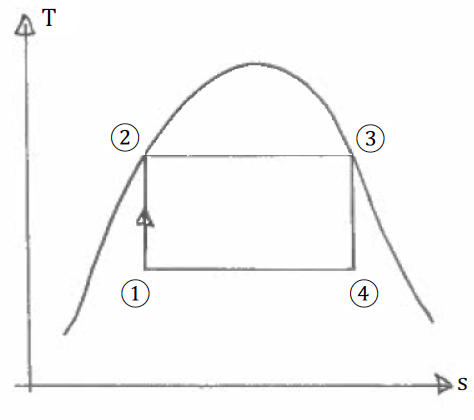
\includegraphics[width=0.5\linewidth]{./figures/f7_1.png}
  \label{fig:f7_1}
\end{figure}
Carnots kredsproces er dog i sin grundessens en teoretisk model. Hvis denne skulle realiseres i virkeligheden vil et par teoretiske udfordringer (som vi endnu ikke har løst) skulle løses. Disse er i hovedtræk:
\begin{itemize}
  \item Tilstand 1-2: Isentropisk trykøgning (f.eks. i en pumpe): Det vil være en udfordring at lave en holdbar pumpe som kan håndtere en to-fase strømning uden at få kaviation i indløbet til pumpen.
  \item Tilstand 3-4: Isentropisk ekspansion (f.eks. i en turbine): Det vil være en udfordring at lave en turbine, som kan håndtere så lave $x$-værdier i bagenden uden, at der ville ske ødelæggende slitage af væskedråber ved de høje strømningshastigheder som der forefindes i bagenden af en turbine.
\end{itemize}

\begin{definition}[Kaviation]
  Kaviation er et begreb for den ødelæggende virkning, der sker ved implosion af gasbobler, som dannes i en væske (som er tæt ved kogepunktet) ved en uundgåelig trykreduktion i indløbet af en pumpe. Når der igen trykopbygges i pumpen, imploderer gasboblerne. Implosion af gasbobler kan føre til pitting (kraterdannelse) i overfladen af pumpehuset og løbehjulet. 
\end{definition}

For at imødekomme de ovenstående problemer foreslog Rankine en modificeret Carnot-proces, som er grafisk afbildet i et $T$-$s$ diagram på \textbf{\autoref{fig:f7_2}} og vist i et eksemplificeret procesdiagram på \textbf{\autoref{fig:f7_3}}. 
\begin{figure} [ht]
  \centering
  \caption{Rankines kredsproces i et $T$-$s$ diagram}
  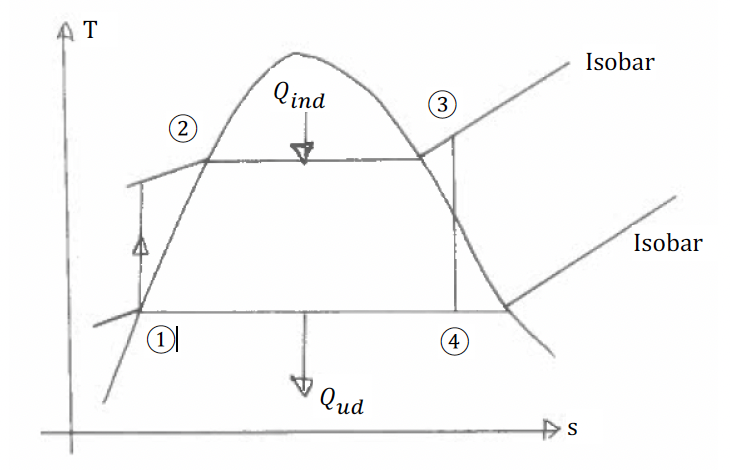
\includegraphics[width=0.5\linewidth]{./figures/f7_2.png}
  \label{fig:f7_2}
\end{figure}
\begin{figure} [ht]
  \centering
  \caption{Procesdiagram for Rankines kredsproces}
  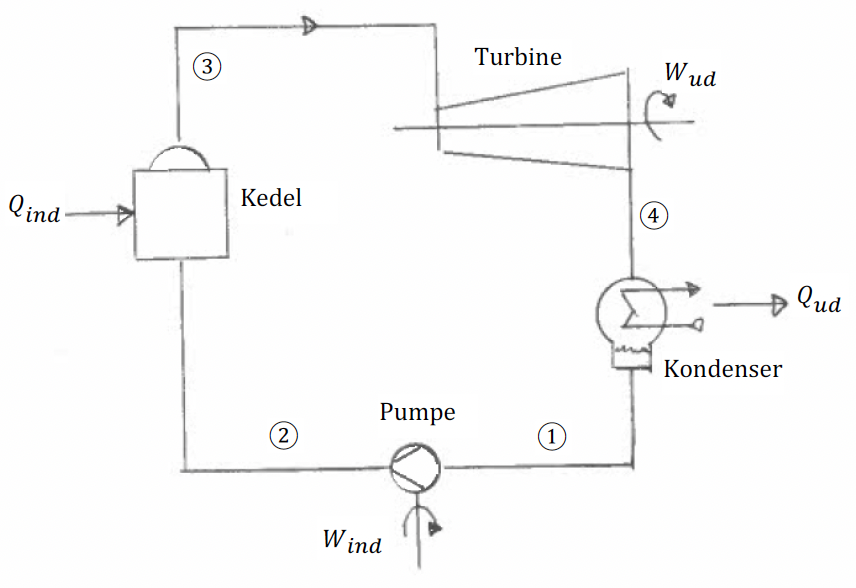
\includegraphics[width=0.5\linewidth]{./figures/f7_3.png}
  \label{fig:f7_3}
\end{figure}
Rankines kredsproces består af følgende delprocesser:
\begin{itemize}
  \item Tilstand 1-2: Isentropisk kompression (pumpe)
  \item Tilstand 2-3: Isobarisk varmetilførsel (kedel)
  \item Tilstand 3-4: Isentropisk ekspantion (turbine)
  \item Tilstand 4-1: Isobarisk varmeafgivelse (kondenser)
\end{itemize}
Det skal selfvølgeligt bemærkes at selvom Rankines kredsproces er et forsøg på at ``afidealisere'' Carnots proces så er Rankine processen stadigt grundlæggende idealiseret idet der ses bort fra tryktab i diverse komponenter og rørforbindelser.

I dette kursus behandles Rankine kredsprocessen ed de to isentropiske delprocesser 1-2 og 3-4, og det forudsættes:
\begin{itemize}
  \item At delprocesserne er reversible, hvilket indebærer at der ikke er friktion og dermed tryktab internt i anlægget
  \item At alle komponenter er adiabatiske -- på nær der, hvor der skal ske varmeveksling -- dvs. at der ikke varmeveksles mellem komponenterne internt eller er utilsigtet varmetab til omgivelserne.
\end{itemize}
Da delprocesserne 1-2 og 3-4 er forudsat isentropiske, vil de også være adiabatiske, hvorfor:
\[ 
Q_{12} = Q_{34} = 0
.\]
Delprocesserne 2-3 og 4-1 er hhv. isobarisk varmetilførsel og -afgivelse for et åbent system og derfor har vi her
\begin{align*}
  Q_{23} &= m \cdot \left( h_3 - h_2 \right) \\
  Q_{41} &= m \cdot \left( h_1 - h_4 \right)
.\end{align*}
Derudover er nettoarbejdet for Rankine processen givet ved
\[ 
W_{\mathrm{net}} = W_{34} + W_{12} = -Q_{\mathrm{net}} = - \left( Q_{23} + Q_{41} \right)
.\]
Den termiske virkningsgrad for den ideelle Rankine-proces kan dernæst defineres som
\[ 
\eta_{th, \mathrm{Rankine}} = \frac{\text{Ønsket output}}{\text{Nødvendigt input}} = \frac{|W_{\mathrm{net}}|}{Q_{23}} = \frac{Q_{23} + Q_{41}}{Q_{23}} = 1 - \frac{|Q_{41}|}{Q_{23}} = 1 - \frac{h_4 - h_1}{h_3 - h_2}
.\]

\subsection{Kraftværket}

\subsubsection{Kraftværkets basiskredsproces}
For at gøre Rankine-kredsprocessen mere virkelighedsnær, indføres den isentropiske virkningsgrad for både pumpe og turbine. Rankine-processen er den mest benyttede på de termiske kraftværker, der benytter vandt som det cirkulerende medie, da det er billigt, tilgængeligt i store mængder og ikke miljøskadeligt. Et typisk kraftværk består således af følgende delprocesser (afbildet på \textbf{\autoref{fig:f7_4}}:
\begin{itemize}
  \item Tilsand 1-2: Kompression (pumpe)
  \item Tilstand 2-3: Isobarisk varmetilførsel (kedel)
  \item Tilstand 3-4: Ekspansion (turbine)
  \item Tilstand 4-1: Isobarisk varmeafgivelse (kondenser)
\end{itemize}
\begin{figure} [ht]
  \centering
  \caption{Rankines kredsproces i et $T$-$s$ diagram med uundgåelige tab i pumpe og turbine}
  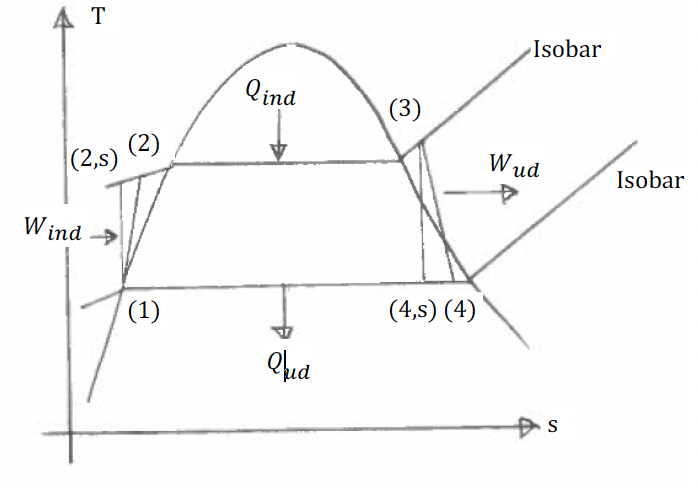
\includegraphics[width=0.5\linewidth]{./figures/f7_4.png}
  \label{fig:f7_4}
\end{figure}

Der fokuseres nu på effekt i stedet for varme, hvilket nemt gøres, idet massen $m$ udskiftes med massestrømmen $\dot{m}$. Bestemmelsen af effekterne i kredsprocessen, idet alle med overlæg beregnes positive, bestemmes ved formlerne:
\begin{align*}
  \dot{W}_{12} &= \dot{m} \cdot \left( h_2 - h_1 \right) \\
  \dot{Q}_{23} &= \dot{m} \cdot \left( h_3 - h_2 \right) \\
  \left| \dot{W}_{34} \right| &= \dot{m} \cdot \left( h_3 - h_4 \right) \\
  \left| \dot{Q}_{41} \right| &= \dot{m} \cdot \left( h_4 - h_1 \right)
.\end{align*}
Massestrømmen af vand som cirkulerer vil være konstant. Det skal i øvrigt bemærkes at arbejdet $\dot{W}$ er det samme som det indre arbejde $\dot{W}_i$ som er summen af det tekniske arbejde $\dot{W}_t$ og dissipationsarbejdet $\dot{W}_{\mathrm{diss}}$. Den termiske virkningsgrad for et kraftværk vil være uforandret:
\begin{equation} \label{eq:virkRan}
  \eta_{th, \mathrm{Rankine}} = 1 - \frac{\left| Q_{41} \right|}{Q_{23}} = 1 - \frac{h_4 - h_1}{h_3 - h_2}
\end{equation}

\begin{figure} [ht]
  \centering
  \caption{Procesdiagram for et kraftværk med forskellige systemgrænser}
  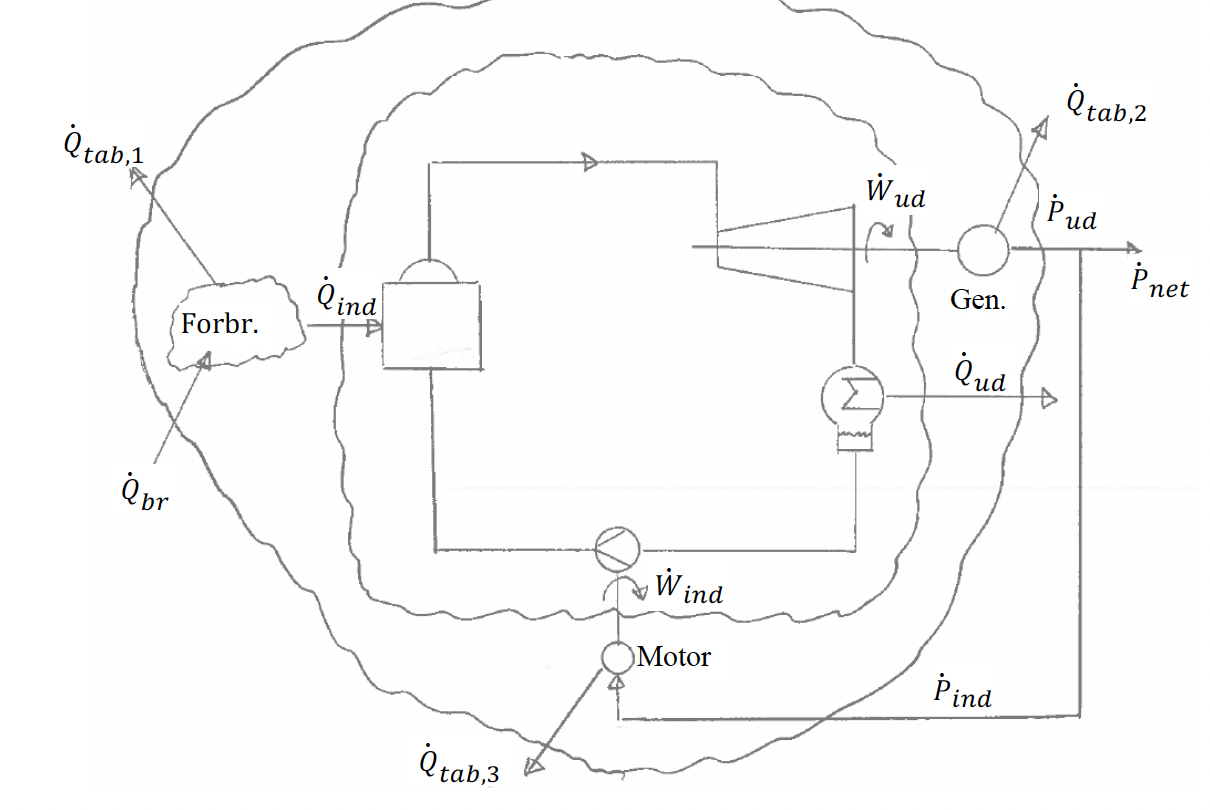
\includegraphics[width=0.5\linewidth]{./figures/f7_5.png}
  \label{fig:f7_5}
\end{figure}
På \textbf{\autoref{fig:f7_5}} er tegnet et procesdiagram for et kraftværk efter Rankine-princippet vist med to forskellige systemgrænser. Den inderste systemgrænse er konsistent med beregningen af den termiske virkningsgrad vist i \textbf{\autoref{eq:virkRan}}. Imidlertid benyttes den termiske virkningsgrad sjældent i praksis, idet den ikke umiddelbart lader sig benytte i en kommerciel situation. 

I praksis benyttes den virkningsgrad som knytter sig til den yderste systemgrænse i \textbf{\autoref{fig:f7_5}} som benævnes den \textit{elektriske virkningsgrad} $\eta_{\mathrm{el}}$ også kaldet den økonomiske virkningsgrad. Forskellen mellem den termiske virkningsgrad $\eta_{th, \mathrm{Rankine}}$ og den elektriske virkningsgrad $\eta_{\mathrm{el}}$, er at den elektriske virkningsgrad medtager de uundgåelige tab, som forefindes i dampkedel, generator/gear og motorer. Afhængigt af om man fokuserer på et generatoroutput $\dot{P}_{\mathrm{ud}}$ eller eksporteret eleffekt til elnettet $\dot{P}_{\mathrm{net}}$ kan defineres en \textit{brutto elektrisk virkningsgrad} $\eta_{el, b}$ eller en \textit{netto elektrisk virkningsgrad} $\eta_{el, n}$. Disse kan findes som:
\begin{align*}
  \eta_{el, b} &= \frac{\text{Ønsket output}}{\text{Nødvendigt input}} = \frac{\left| \dot{P}_{\mathrm{ud}} \right|}{\dot{Q}_{br}} = \frac{\left| \dot{P}_{\mathrm{ud}} \right|}{\dot{m}_{br} \cdot \mathrm{LHV}} \\
  \eta_{el, n} &= \frac{\text{Ønsket output}}{\text{Nødvendigt input}} = \frac{\left| \dot{P}_{\mathrm{net}} \right|}{\dot{Q}_{br}} = \frac{\left| \dot{P}_{\mathrm{ud}} \right| - \dot{P}_{\mathrm{ind}}}{\dot{m}_{br} \cdot \mathrm{LHV}}
.\end{align*}
Disse er mere anvendelige i praksis, da både tæller og nævner direkte kan relateres til økonomiske parametre i et regnskab.


\subsubsection{Fødevandsforvarming}
Kraftværkets basiskredsprocess som vist på \textbf{\autoref{fig:f7_5}} ville kunne fungere i praksis, men for at undgå ophobning af gasser herunder ilt og kuldioxid stammende fra spædevand eller lækager i kredsløbet, er man nødt til at aflufte det cirkulerende vand. Til dette benyttes en fødevandstank med aflufterfunktion. Fødevandstanken tjener i praksis som fødevandsbuffer for dampkedlen. På \textbf{\autoref{fig:f7_6}.a} er basisprocessen med fødevandstank vist, og på \textbf{\autoref{fig:f7_6}.b} er vist et procesdiagram for en fødevandstank med aflufterfunktion. 
\begin{figure} [ht]
  \centering
  \caption{Procesdiagram for et kraftværk med en fødevandstank}
  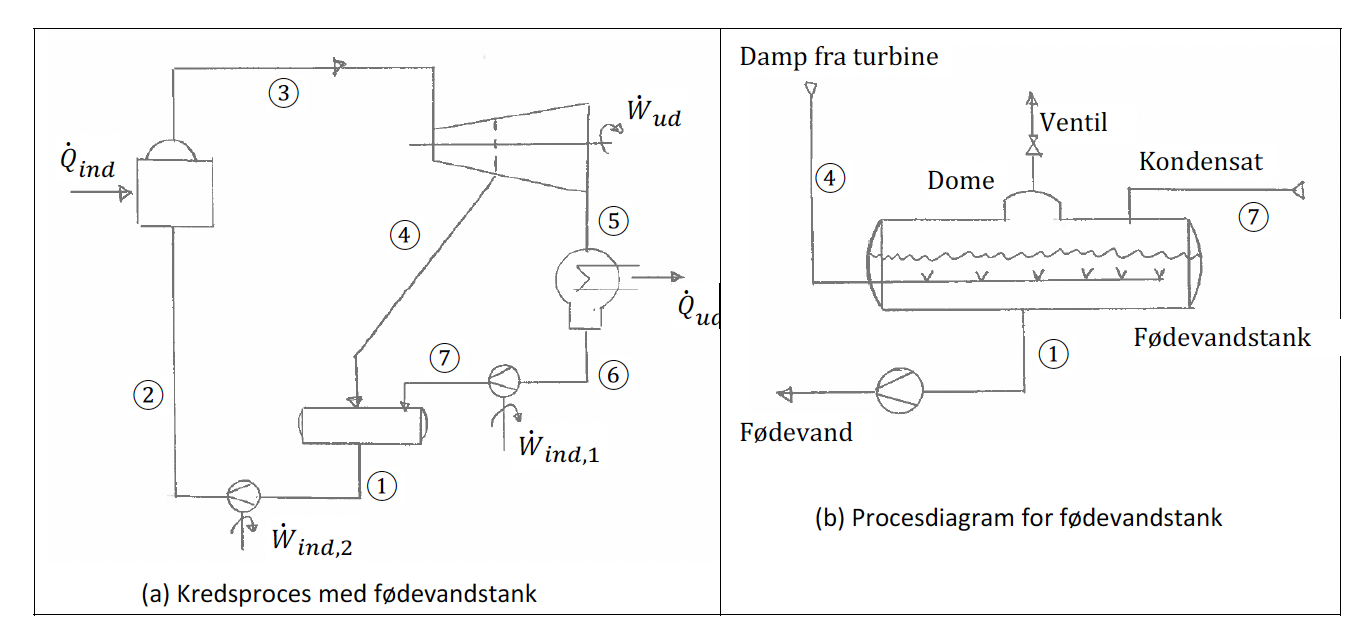
\includegraphics[width=0.5\linewidth]{./figures/f7_6.png}
  \label{fig:f7_6}
\end{figure}

Fødevandstanken er i bund og grund en varmeveksler, hvor der sker opblanding af medier. Damp udtaget fra turbinen til opvarme vandet i fødevandstanken til mætningstemperaturen for det tryk dampen har. Ved opvarmning uddrives gasser, som samles i domen og lukkes ud til atmosfæren igennem en mindre ventil på toppen af domen. Princippet kaldes \textit{termisk afluftning}, og det kendes fra køkkenet, hvor den syngende lyd, som kommer fra en vandkedel under opvarmning i temperaturområdet \qty{60}{\celsius}--\qty{90}{\celsius}, netop stammer fra uddrivning af gasser fra postevandet.

Vandet i fødevandstanken vil være på kogepunktet, dvs. $x=0$. Trykket i fødevandstanken er bestemt af trykket på dampen fra dampturbinen. Dette tryk kan man selv bestemme ved at utablere et udtag når man bygger dampturbinen. Der hvor udtaget er etableret, kan man aflæse dampens tilstand på turbineekspansionskurven. I et $h$-$s$ diagram er det skæringspunktet mellem isobaren ved udtaget og turbineekspansionskurven.

Som det ses i \textbf{\autoref{fig:f7_6}.b} vil der være brug for to pumper. Mediet (vandet) mellem kondenseren og fødevandstanken benævnes turbinekondensat, hvorfor pumpen der benævnes \textit{kondensatpummpen}. Mediet (vandet) efter fødevandstanken kaldes \textit{kedelfødevand}, hvorfor pumpen der benævnes \textit{kedelfødevandspumpen}. 

Populært siger man, at man stjæler lidt varme fra turbinen og benytter det til at forvarme kedelfødevandet. Den dampmængde man optager fra turbinen har allerede bidraget til akseleffekt i turbinen og restvarmen i dampen, som overføres til kedelfødevandet, vil resultere i et reduceret brændstofforbrug i kedlen. Dettte benævnes \textit{regenerativ fødevandsforvarmning}, og har en positiv effekt på virkningsgraden for den samlede proces.

Fødevandstanken kan beregnes som et knudepunkt (se evt. \textbf{\autoref{afs:knude}}). Idet man ser bort fra negligerbare forhold ved ventilen på toppen af domen kan opstilles følgende:
\begin{align*}
  \dot{m}_7 \cdot h_7 + \dot{m}_4 \cdot h_4 &= \dot{m}_1 h_1 \\
  \dot{m}_7 + \dot{m}_4 &= \dot{m}_1
.\end{align*}
Som kan kombineres til
\[ 
\dot{m}_4 = \dot{m}_7 \cdot \frac{h_1 - h_7}{h_4 - h_1}
.\]
Herved kendes den dampmængde, som skal udtages af dampturbinen. Akseleffekten fro turbinen kan derefter bestemmes ved formel:
\[ 
\left| \dot{W}_{\mathrm{ud}} \right| = \left| \dot{W}_i \right| = \dot{m}_3 \cdot (h_3 - h_4) + (\dot{m}_3 - \dot{m}_4) \cdot (h_4 - h_5)
.\]

\subsubsection{Turbinekondenser}
Kondenseren ved dampturbinen er et centralt komponent i kraftværket. Kondenseren er en varmeveksler, hvor der ikke sker opblanding af medierne. Et procesdiagram for dette er vist på \textbf{\autoref{fig:f7_7}}.
\begin{figure} [ht]
  \centering
  \caption{Procesdiagram for en turbinekondenser}
  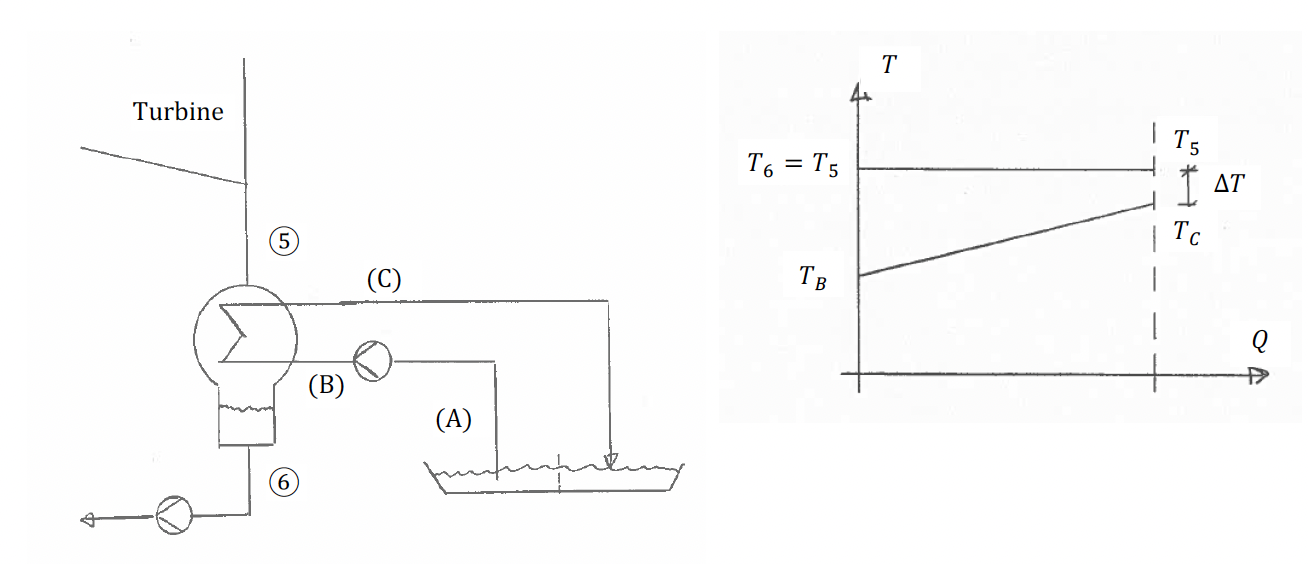
\includegraphics[width=0.5\linewidth]{./figures/f7_7.png}
  \label{fig:f7_7}
\end{figure}
Damp fra dampturbinen ledes til kondenseren i pkt. 5, hvor det kondenserer til vand (kondensat) i pkt. 6. Effekten overført fra den kondenserede damp bestemmes ved formlen:
\[ 
\left| \dot{Q}_{41} \right| = \dot{m} \cdot \left( h_4 - h_1 \right)
.\]
Kondensatet opsamles i en tank kaldet \textit{hotwell} under kondenseren. Kondenseren kan køles af en række medier, som f.eks. havvand, fjernvarmevand eller luft. Antages her, at køling sker med vand, kan effektbalance for kølevandet bestemmes af formlen:
\[ 
\left| \dot{Q}_{56} \right| = \left| \dot{Q}_{BC} \right| = \dot{m}_{\text{kølevand}} \cdot (h_C - h_B) = \dot{m}_{\text{kølevand}} \cdot c_{p,m} \cdot \left( T_C - T_B \right)
.\]
For vand kan man tilnærmelsesvist sætte den specifikke varmekapacitet til $c_{p,m} = \qty{4,19}{\frac{kJ}{kgK}}$. Køle\-vands\-mæng\-den kan således, hvis det antages, at der ikke er varmetab bestemmes som:
\[ 
\dot{m}_{\text{kølevand}} = \frac{\left| \dot{Q}_{BC} \right|}{h_C - h_B} = \frac{\left| \dot{Q}_{56} \right|}{h_C - h_B}
.\]
Det er kondenseren som bestemmer trykket efter turbinen. Med reference til \textbf{\autoref{fig:f7_7}} vil det være $T_C$ som sætter temperaturen i kondenseren eller udtrykt som en formel som
\[ 
T_5 = T_C + \Delta T
.\]
$\Delta T$ er i praksis \qty{2}{\celsius}--\qty{4}{\celsius}. Ved $\Delta T = \qty{0}{\celsius}$ skulle kondenserens areal være uendeligt stort. I damprummet kendes nu temperaturen $T_5$, og da der er entydig sammenhæng mellem temperatur og tryk ved kondensation, kan man slå damptrykket op i bogens Appendiks D5 under mættet tilstand. 


\subsection{Kraftvarmeværket}
Kraftvarmeværket er ligeledes baseret på Rankine-princippet. Eneste forskel er at man foruden netto-eleffekten $\dot{W}_{\mathrm{net}}$ ligeledes anser varmeeffekten fra kondenseren $\dot{Q}_{41}$ for nyttig. Varmeeffekten fra kondenseren kan være nyttig, hvis den f.eks. sælges som fjernvarme.

For kraftvarmeværket (KKV) kan defineres en termisk virkningsgrad som:
\[ 
\eta_{th, \mathrm{Rankine, KKV}} = \frac{\text{Ønsket output}}{\text{Nødvendigt input}} = \frac{\left| W_{\mathrm{net}} \right| + \left| Q_{41} \right|}{Q_{23}} = \frac{Q_{23}}{Q_{23}} = 1
.\]
Den termiske virkningsgrad for et KKV er altså i princippet 1 eller 100\%. Dette gælder dog ikke den elektriske virkningsgrad. For et KKV benævnes denne dog som den totale virkningsgrad og denne kan findes som:
\begin{align*}
  \eta_{\mathrm{total}, b} &= \frac{\text{Ønsket output}}{\text{Nødvendigt input}} = \frac{\left| \dot{P}_{\mathrm{ud}} \right| + \left| \dot{Q}_{41} \right|}{\dot{Q}_{br}} = \frac{\left| \dot{P}_{\mathrm{ud}} \right| + \left| \dot{Q}_{41} \right|}{\dot{m}_{br} \cdot \mathrm{LHV}} \\
  \eta_{\mathrm{total}, n} &= \frac{\text{Ønsket output}}{\text{Nødvendigt input}} = \frac{\left| \dot{P}_{\mathrm{net}} \right| + \left| \dot{Q}_{41} \right|}{\dot{Q}_{br}} = \frac{\left| \dot{P}_{\mathrm{ud}} \right| - \dot{P}_{\mathrm{ind}} + \left| \dot{Q}_{41} \right|}{\dot{m}_{br} \cdot \mathrm{LHV}}
.\end{align*}
Tabene i dampkedlen, generator/gear og motorer vil afstedkomme, at totalvirkningsgraden ikke bliver 1 men derimod i praksis ligger i intervallet \num{0,85}--\num{0,95}.

\subsection{Optimering af Rankine kredsprocessen} \label{afs:optRan}
Med udgangspunkt i den termiske virkningsgrad for Rankine princippet kan der uddrages en række interessante konklusioner. Generelt har vi at:
\[ 
\eta_{th, \mathrm{Rankine}} = 1 - \frac{h_4 - h_1}{h_3 - h_2}
.\]
\begin{enumerate}
  \item Hvis entalpien af dampen før turbinen $h_3$ stiger, vil den termiske virkningsgrad for Rankineprocessen $\eta_{th, \mathrm{Rankine}}$ stige. Dette kan udføres, hvis damptryk og/eller temperatur sættes op.
  \item Hvis entalpien af dampen efter turbinen $h_4$ falder, vil den termiske virkningsgrad $\eta_{th, \mathrm{Rankine}}$ stige. Dette kan udføres, hvis trykket i kondenseren sænkes.
\end{enumerate}

Derudover kan det vises at følgende tiltag også øger den termiske virkningsgrad:
\begin{itemize}
  \item Øge fødevandstemperaturen før dampkedlen vha. regenerativ fødevandsforvarmning
  \item Ved fastsat fødevandstemperatur før dampkedlen at udføre regenerativ fødevandsforvarmnning i så mange trin som muligt, dvs. så mange fødevandsforvarmere som muligt
  \item Dele turbinen i to sektioner, og genoverhede (også kaldet mellemoverhede) dampen i dampkedelen mellem de to turbinesektioner
\end{itemize}

\subsection{Organic Rankine Cycle (ORC)}
Rankine-processen benyttes til at konvertere varme til arbejde. Traditionelt har man brugt fossile brændsler som kul, olie og naturgas som energikilde. Ved forbrænding af disse materialer kan man nemt opnår forbrændingstemperaturer $> \qty{1200}{\celsius}$, som er rigeligt for en højeffektiv Rankine-proces. Det er ikke forbrændingstemperaturen, som sætter begrænsnignerne for en høj virkningsgrad på et kraftværk, men derimod tilgængelige materialer til overhederør i dampkedlen, hoveddampledningen og dampturbinens første trin. Grænsen er i dag ca. \qty{300}{bara} og \qty{600}{\celsius}.

Man kan dog også benytte Rankine-processen til at udnytte visse lav-temperatur varmekilder, såsom solenergi, geotermisk energi og spildvarme fra procesindustrien. For energikilder med en temperatur på $< \qty{100}{\celsius}$ ville man få et teknisk problem med Rankine-processen baseret på vand. Trykket overalt i anlægget ville her skulle være under atmosfæretrykket, hvorfor der ved lækager vil trænge luft og dermed ilt ind i systemet -- derfor benytter man typisk et andet medie i denne situation.

Et anlæg, der baserer sig på Rankine-princippet og indeholder et organisk medie benævnes et \textit{Organic Rankine Cycle anlæg} eller forkortet til ORC-anlæg. Disse benyttes typisk i praksis for anlæg med temperaturer mellem \qty{50}{\celsius} og \qty{350}{\celsius}. Man skal dog i denne sammenhæng ikke regne med et særligt effektivt procesforløb eftersom man med en lav temperatur får en dårlig Carnot-virkningsgrad.
\[ 
\eta_{th, C} = 1 - \frac{T_L}{T_H}
.\]

I et ORC-anlæg benyttes typisk:
\begin{itemize}
  \item Organiske kølemidler
  \item Organiske brændbare gasser
  \item Ammoniak
\end{itemize}
Ammoniak er egentligt ikke organisk, men det er intet desto mindre brugbart på lige fod med de egentligt organiske materialer. Når man designer et ORC-anlæg og vælger sit medie kan man inddrage følgende prioriterede kriterier:
\begin{enumerate}
  \item Den termiske virkningsgrad skal være så høj som muligt
  \item Tryk i kondenseren bør være så lavt som muligt, og helst højere end atmosfæretrykket
  \item Tryk i kedlen bør være så lavt som muligt
\end{enumerate}

ORC-anlæg har en afgørende forskel ift. vandbaserede KVV'er. Som det ses på \textbf{\autoref{fig:f7_8}.a} benyttes restvarmen i det cirkulerende medie efter turbinen til at forvarme væsken som ledes til kedlen. Dette skyldes den form på ``osteklokken'' som er typisk for et organisk stof. På \textbf{\autoref{fig:f7_8}.b} er vist et typisk procesforløb i et $p$-$h$ diagram. Efter ekspansion af den overhedede gas i turbinen, vil gassen efter turbinen stadig være overhedet i en sådan grad, at det vil være opportunt at genanvende overhedningsvarmen i kedlen -- for derved at spare på varmetilførslen til kedlen. Alterneativt ville være en simpel bortkøling af overhedningsvarmen i kondenseren og en ringere termisk virkningsgrad.

\begin{figure} [ht]
  \centering
  \caption{Processdiagram og tilstandsdiagram for et typisk ORC-anlæg}
  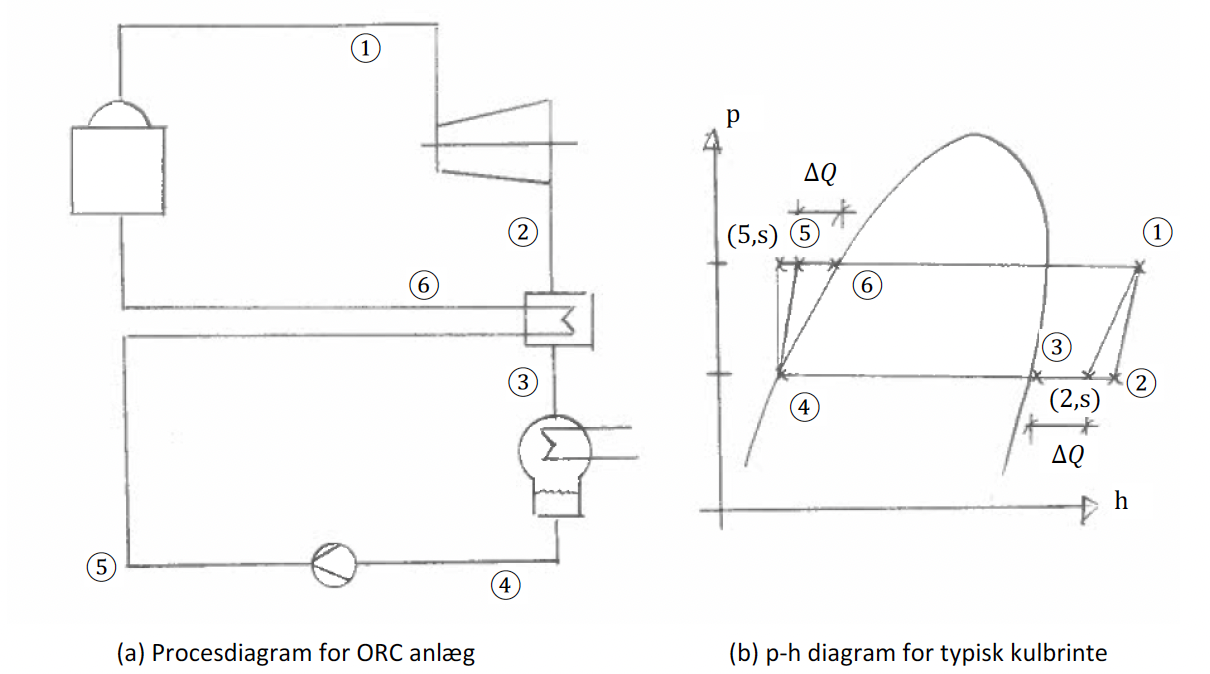
\includegraphics[width=0.5\linewidth]{./figures/f7_8.png}
  \label{fig:f7_8}
\end{figure}


\subsection{Samlet Brayton og Rankine kredsprocess -- Kombineret proces}
Gasturbiner er kendetegnet ved at frembringe en stor akseleffekt i forhold til deres vægt. Typisk trækker en landbaseret gasturbine en generator som producerer strøm. Røggas-afgangstemperaturen fra en gasturbine er typisk \qty{500}{\celsius}--\qty{600}{\celsius}, hvilket giver typiske virkningsgrader for en gasturbine på 35--50\%. Kobles en dampkedel efter en gasturbine vil man kunne køle røggassen ned til \qty{150}{\celsius}--\qty{200}{\celsius}, og dampen kunne ekspanderes i en dampturbine med henblik på at producere yderligere elektrisk energi. Et procesdiagram for et kombineret gasturbine- og dampkraftværk eller med andre ord et kombineret Brayton og Rankine anlæg er vist på \textbf{\autoref{fig:f7_9}}. 

\begin{figure} [ht]
  \centering
  \caption{Procesdiagram for et kombineret Brayton og Rankine anlæg}
  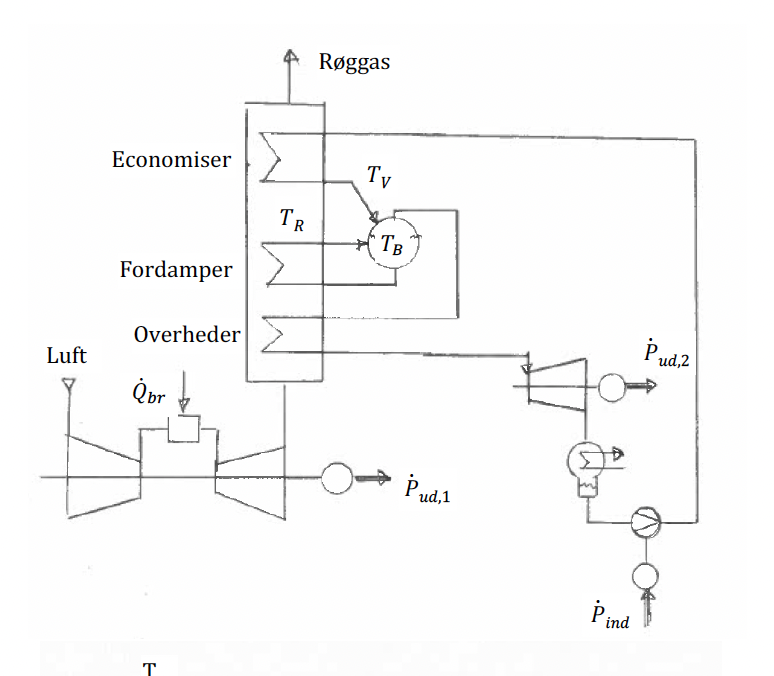
\includegraphics[width=0.5\linewidth]{./figures/f7_9.png}
  \label{fig:f7_9}
\end{figure}

Dampkedlen, som i fagsprog kaldes en \textit{udstødskedel} eller en \textit{afgaskedel}, er opbygget traditionelt med en fordamper, overheder og economiser. Til beregninger på denne kan de tidligere introducerede formler for dampkedler benyttes. Både economiser og overheder er arrangeret på en sådan måde, at hhv. vandet eller dampen strømmer i modstrøm til røggassen, hvilket giver den bedste mulighed for effektiv afkøling af røggassen. Strømningsretningen af det kogende vand i fordamperen er dog i medstrøm med røggassen, hvilket skyldes, at man ønsker, at strømningsretningen af en kogende væske er opad.. De dannede dampbobler kan strømme modstrøms op i dampbeholderen. Opadstigende dampbobler i en nedadstrømmende kogende væske kan give anledning til voldsomme vibrationer i anlægget. De opadstigende bobler vil også medfører et termisk løft, hvorfor man kan opnå naturcirkulation af vandet i fordamperen og derved spare en cirkulationspumpe. 

Røggassens strømning igennem dampkedlen vil naturligvis afstedkomme et tryktab, som gasturbinen skal overvinde, hvilket vil påvirke gasturbinens ydelse -- dog oplyser mange gasturbineleveerandører data for gasturbinens drift med den forudsætning, at der tillades et trykfald efter gasturbinen på op til \qty{30}{mbar} eller \qty{3000}{Pa}, hvilket normalt er rigeligt til at kunne designe en egnet udstødskedel.

\begin{figure} [ht]
  \centering
  \caption{$Q$-$T$ diagram for et kombineret Brayton og Rankine anlæg}
  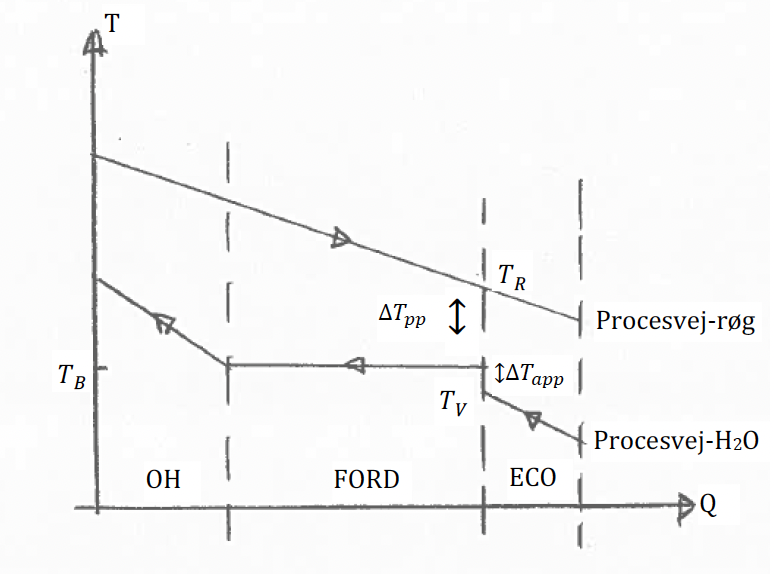
\includegraphics[width=0.5\linewidth]{./figures/f7_10.png}
  \label{fig:f7_10}
\end{figure}

På \textbf{\autoref{fig:f7_10}} ses et $Q$-$T$ diagram for et kombineret Brayton og Rankine anlæg. Med afsæt i dette fremhæves en række karakteristike ved en afgaskedel:
\begin{enumerate}
  \item I \textbf{\autoref{afs:optRan}} konkluderedes, at temperaturen på dampen før en dampturbine skal være så høj som muligt for at maksimere virkningsgraden for en Rankine proces. Dampafgangstemperaturen for en afgaskedel kan ikke overstige temperaturen på røggassen, som leveres af gasturbinen. Er røggastemperaturenn leveret af gasturbinen \qty{550}{\celsius}, vil en kommercielt afbalanceret dampafgangstemperatur være ca. \qty{520}{\celsius}. En temperaturdifferent mellem røggastilgangstemperatur og dampafgangstemperatur for en overheder arrangeret i modstrøm på \qty{25}{\celsius}--\qty{35}{\celsius}, vil resultere i en overheder med et varmeoverførende areal som er fornuftigt, når både anlægspris og driftsindtægter tages i betragtning.
  \item I \textbf{\autoref{afs:optRan}} konkluderedes ligeledes, at tryk på dampen før en dampturbine skal være så høj som muligt for at maksimere virkningsgraden på en Rankine-proces. Røggastemperaturen efter fordamperen ($T_R$ på \textbf{\autoref{fig:f7_10}}) er dog direkte afhængig af det valgte damptryk, idet der i fordamperen sker kogning, hvorfor tryk og temperatur er entydigt sammenhængende. Vælges damptrykket til f.eks. \qty{10}{bara} vil temperaturen i fodamperen ($T_B$ på \textbf{\autoref{fig:f7_10}}) være konstant \qty{180}{\celsius}. Temperaturdifferensen $\Delta T_{pp}$ mellem røggastemperaturen efter fordamperen $T_R$ og temperatur i fordamperen $T_B$ benævnes i international litteratur for \textit{pinch point} og er i praksis \qty{10}{\celsius}--\qty{15}{\celsius}, og størrelsen har signifikant indflydelse på prisen på afgaskedlen. Jo lavere damptryk desto lavere røggastemperatur efter fordamperen, hvilket er ønskeligt ud fra en betragtning af at skulle køle røggassen mest muligt, men er i modstrid med at damptrykket skal være så højt som muligt for at få den højeste virkningsgrad på Rankine-processen alene.
  \item Man kunne hævde at den energi, som ikke kan optages i overhederen og fordamperen, kunne optages i economiseren. Men kølekapaciteten af economiseren er begrænset af to faktorer. For det første vil vandmængden igennem economiseren være begrængset til dampmængden. For det andet ønskes ikke kogning i vandet i eller efter economiseren. Dette er et gammeldags princip indenfor kedelbygning og grundes i at dampdannelse vil skabe vibrationer. I praksis begrænser man temperaturen på vandet efter economiseren ($T_V$ på \textbf{\autoref{fig:f7_10}}) til \qty{5}{\celsius} under temperaturen i fordamperen $T_B$. Temperaturdifferensen $\Delta T_{app}$ mellem temperaturen i fordamperen $T_B$ og temperaturen på vandet efter economiseren $T_V$ benævnes i international litteratur for \textit{approach point}. 
\end{enumerate}

Hvis man ønsker at få røggastemperaturen efter anlægget længere ned end ca. \qty{150}{\celsius}--\qty{200}{\celsius} (afhængigt af $T_B$) kan man sætte to eller tre (eller flere) kedler ovenpå hinanden. Ved tre dampkedler kunne de producere damp ved hhv. 80, 10 og \qty{2}{bara}. Dampen kunne tilflyde den samme dempturbine, en forskellige steder ift. turbineekspansionskurven. Damp genereret ved de 10 og \qty{2}{bara} kunne tilsættes igennem huller i turbinehuset, hvor dampen i turbinen har samme tryk jf. turbineekspansionskurven. Et damptryk på \qty{2}{bara} i den sidste fordamper, ville muliggøre en røggastemperatur efter selvsamme på $\qty{120}{\celsius} + \Delta T_{pp} = 130 - \qty{135}{\celsius}$. Yderligere afkøling af røggassen i den sidste economiser på \qty{10}{\celsius}--\qty{15}{\celsius} ville give en røggastemperatur på ca. \qty{120}{\celsius}--\qty{125}{\celsius}.

En praktisk fremgangsmåde for bestemmelse af en masse- og energibalance for kedeldelen vil være at lægge en imaginær systemgrænse rundt om dampbeholderen, fordamperen og overhederen. Røggastemperaturen efter fordamperen vil være mætningstemperatur i dampbeholderen $T_B$ plus $\Delta T_{pp}$ og effekten afgivet til systemeet kan bestemmes, da røggastemperaturen efter gasturbinen bør være kendt. På vand/dampsiden kendes entalpidifferensen mellem fødevand før dampbeholderen (Temperaturen her er $T_B - \Delta T_{app}$) og damp efter overhederen. Herved kan dampmassestrømmen bestemmes, og de resterende beregninger på vand/dampkredsen kan færdiggøres ved bla. at lægge yderligere imaginære systemgrænser.
